\iffalse
\title{Assignment}
\author{EE24BTECH11038}
\section{xe}
\chapter{2007}
\fi
\item Match the conventional ceramic materials listed in Column I with their respective common applications in Column II

\begin{tabular}{|c|c|}
\hline
\textbf{Column I} & \textbf{Column II} \\
\hline
P. Lead Zirconate Titanate (PZT) & 1. cutting tool \\
Q. Zinc Oxide (ZnO) & 2. thermal barrier coating \\
R. Silicon Carbide (SiC) & 3. actuator \\
S. Zirconia (ZrO$_2$) & 4. varistor \\
 & 5. super conductor \\
\hline
\end{tabular}

\begin{enumerate}
    \item P-1, Q-2, R-3, S-5
    \item P-3, Q-2, R-1, S-5
    \item P-2, Q-1, R-5, S-3
    \item P-3, Q-4, R-1, S-2
\end{enumerate}
\bigskip 
\item Match the terminologies given in Column I with their relations listed in Column II
\begin{tabular}{|c|c|}
\hline
\textbf{Column I} & \textbf{Column II} \\
\hline
P. domain wall & 1. superconductors \\
Q. Fick's law & 2. mechanical properties \\
R. Matthiessen's rule & 3. ferromagnetic materials \\
S. Hall-Petch relation & 4. resistivity of impure metals \\
T. Meissner effect & 5. diffusion \\
\hline
\end{tabular}
\begin{enumerate}
    \item P-1, Q-3, R-5, S-2, T-4 
    \item P-3, Q-5, R-2, S-4, T-1
    \item P-3, Q- 5, R-4, S-2, T-1
    \item P-3, Q-4, R-3, S-2, T-4
\end{enumerate}
\bigskip
\item Match the microscopes listed in Column I with their principle of operation listed in Column II
\begin{tabular}{|c|c|}
\hline
\textbf{Column I} & \textbf{Column II} \\
\hline
P. Scanning Electron Microscope (SEM) & 1. van der Waals forces between atoms \\
Q. Transmission Electron Microscope (TEM) & 2. electrons to jump across a potential barrier \\
R. Scanning Tunnelling Microscope (STM) & 3. diffraction of electrons \\
S. Atomic Force Microscope (AFM) & 4. detection of secondary electrons \\
 & 5. photo emission of electrons \\
\hline
\end{tabular}
\begin{enumerate}
    \item P-2, Q-5, R-3, S-1
    \item P-3, Q-4, R-5, S-2
    \item P-4, Q-3, R-2, S-1 
    \item P-4, Q-3, R-5, S-2
\end{enumerate}
\bigskip
\item X-rays of unknown wavelength are diffracted by an FCC metal with a lattice parameter of 0.352nm. The measured `2$\theta$' angle for the {200} peak is 61.08$\degree$. Calculate the wavelength of the X-ray used, in nm
\bigskip
\item A metal with HCP crystal structure has lattice constants a = 0.30 nm and c = 0.56 nm. Determine the volume of the unit cell of this metal, in nm$^3$. 
\bigskip
\item The band gap of a semiconducting material used to make an LED is 1.43 eV. What will be the minimum wavelength of the radiation emitted by this LED, in $\mu$m?
\bigskip
\item For automatic control of household electric water heater a relay switch is activated by thermal expansion of a brass rod of length 50 cm as shown in the schematic below. The distance between the rod and the lever, x, is adjusted by moving the base of the rod. As the water gets heated the rod expands and as soon as the rod touches the lever, the circuit is broken disconnecting the heater from the power supply. Find the distance, x, in mm, to be set at water temperature of 20$\degree$C such that the circuit is broke at 70$\degree$C. The coefficient of linear thermal expansion of brass is 20 x 10$^{-6}$ $\degree$C$^{-1}$ \\

\begin{circuitikz}
    % Main connections and boxes
    \draw (4.25,15.75) -- (4.25,13.5);
    \draw (4.25,13.5) -- (5.5,13.5);
    \draw (5.5,13.75) rectangle (8.25,13.25);
    \draw (7.75,14) rectangle (8,13.75);
    \draw (7.75,14.25) rectangle (13,14);

    % Resistor and short lines
    \draw (12,14.25) -- (12,13) -- (12,11.75);
    \draw (12,11.75) to[R] (12,9.25);
    \draw (8.5,8.25) -- (12,8.25);
    \draw (10,13) rectangle (10.5,8.25);

    % Dashed lines and arrow
    \draw[dashed] (10.5,13) -- (14.25,13);
    \draw[dashed] (13,14.25) -- (14.5,14.25);
    \draw[<->, >=Stealth] (14.25,14.25) -- (14.25,13);

    % Labels
    \node[font=\Large] at (8.5,10.25) {Brass rod};
    \node[font=\Large] at (14.75,13.75) {X};

    % Voltage and AC source lines
    \draw (4.25,15.75) -- (16.25,15.75);
    \draw (15.5,14.25) -- (15.5,9.5);
    \draw (12,9.25) -- (15.5,9.25);
    \draw (15.5,9.25) -- (15.5,10);
    \draw (15.5,14.25) -- (16.25,14.25);

    % Voltage and AC labels
    \node[font=\LARGE] at (15.75,16.25) {230V};
    \node[font=\LARGE] at (16,13.5) {AC};
\end{circuitikz}
 
\bigskip 
\textbf{Common Data Questions}\\
Common Data for Questions 60 and 61:\\

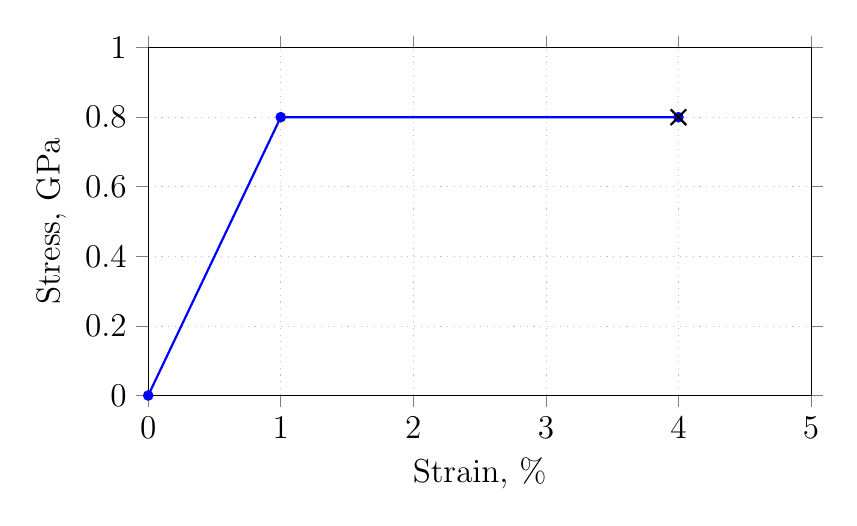
\begin{tikzpicture}
\begin{axis}[
    width=10cm, height=6cm,
    xlabel={Strain, \%},
    ylabel={Stress, GPa},
    xmin=0, xmax=5,
    ymin=0, ymax=1,
    xtick={0,1,2,3,4,5},
    ytick={0,0.2,0.4,0.6,0.8,1.0},
    grid=both,
    major grid style={line width=.2pt,draw=gray!50},
    minor grid style={line width=.1pt,draw=gray!20},
    grid style=dotted,
    tick align=outside
]

% Draw the line
\addplot[blue, thick, mark=*, mark options={fill=blue}, mark size=1.5pt] coordinates {
    (0,0)
    (1,0.8)
    (4,0.8)
};

% Add the final point with a cross
\addplot[black, thick, mark=x, mark options={scale=2, black}] coordinates {(4,0.8)};

\end{axis}
\end{tikzpicture}
From tensile test of a particular alloy the following values were obtained. The material exhibits linear work hardening as shown in the figure given above.

\begin{tabular}{|c|c|c|}
        \hline
        & \textbf{At Yield} & \textbf{At Fracture} \\ \hline
        \textbf{Stress, GPa} & 0.7 & 0.8 \\ \hline
        \textbf{Strain, \%} & 1 & 4 \\ \hline
\end{tabular}


lindrical specimen had a dimension of diameter 10 mm and length 50 mm, find the length of the specimen at the yield point, in mm
\bigskip
\item Find the toughness of the material, in M J m${-3}$\\
\bigskip
\\
Common Data for Questions 62 and 63:\\
An isomorphous alloy system contains 47 wt\% of A and 53 wt \% of B and is at 1300$\degree$ C. Referring to the figure given below, answer the following:
\item What is the weight percentage of A in solid phase at this temperature?

\begin{circuitikz}
\tikzstyle{every node}=[font=\large]
\draw [line width=1.5pt, short] (7.5,16) -- (7.5,6);
\draw [line width=1.4pt, short] (7.5,6) -- (19.25,6);
\draw [short] (7.5,12.25) -- (18.75,12.25);
\draw [short] (7.5,8.5) -- (18.75,14.75);
\draw [short] (7.5,8.5) .. controls (13,14) and (15.25,13.75) .. (18.75,14.75);
\draw [short] (7.5,16) -- (19,16);
\draw [short] (18.75,16) -- (18.75,6.25);
\node [font=\large] at (9.25,13.25) {\textit{\textbf{Liquid}}};
\node [font=\large] at (16.5,8.75) {\textit{\textbf{Solid}}};
\draw [dashed] (12,12.25) -- (12,6);
\draw [dashed] (13.75,16) -- (13.75,6.25);
\draw [dashed] (14.25,12.25) -- (14.25,6);
\draw [short] (7.5,16) -- (7.25,16);
\draw [short] (7.5,14.25) -- (7.25,14.25);
\draw [short] (7.5,12.25) -- (7.25,12.25);
\draw [short] (7.5,10.75) -- (7.25,10.75);
\draw [short] (7.5,8.75) -- (7.25,8.75);
\draw [short] (8.25,6) -- (8.25,5.75);
\draw [short] (9.25,6) -- (9.25,5.75);
\draw [short] (10.25,6) -- (10.25,5.75);
\draw [short] (11.5,6) -- (11.5,5.75);
\draw [short] (13.25,6) -- (13.25,5.75);
\draw [short] (14.5,6) -- (14.5,6);
\draw [short] (14.5,6) -- (14.5,5.75);
\draw [short] (15.5,6) -- (15.5,5.75);
\draw [short] (16.25,6) -- (18.25,6);
\draw [short] (16.5,6) -- (16.5,5.75);
\draw [short] (17.5,6) -- (17.5,5.75);
\node [font=\large] at (6.5,15.75) {1500};
\node [font=\large] at (6.5,14.25) {1400};
\node [font=\large] at (6.5,12.25) {1300};
\node [font=\large] at (6.5,10.75) {1200};
\node [font=\large] at (6.5,8.75) {1100};
\node [font=\large] at (6.5,6.25) {1000};
\node [font=\large] at (18.75,5.25) {100};
\node [font=\large] at (17.5,5.25) {90};
\node [font=\large] at (16.5,5.25) {80};
\node [font=\large] at (15.5,5.25) {70};
\node [font=\large] at (14.5,5.25) {60};
\node [font=\large] at (13.25,5.25) {50};
\node [font=\large] at (11.5,5.25) {40};
\node [font=\large] at (10.25,5.25) {30};
\node [font=\large] at (8.25,5.25) {10};
\node [font=\large] at (9.25,5.25) {20};
\end{circuitikz}

\bigskip
\item What weight percentage of this alloy is liquid?
\bigskip
Statement for Linked Answer Questions 64 and 65:\\
A stress of 10 MPa is applied to an elastomer to generate a strain of 50\%. The strain is held constant at this
value. After 40 days at 20$\degree$C, the stress decreases to 5 MPa\\

\item What is the relaxation time constant for this material?
\bigskip
\item What will be the stress after 60 days at 20$\degree$C?

